\documentclass[aspectratio=169,10pt]{ctexbeamer}

\usetheme{Madrid}
\usecolortheme{default}
\setbeamertemplate{navigation symbols}{}
\setbeamertemplate{itemize items}[circle]
\setbeamertemplate{enumerate items}[default]

\usepackage{amsmath}
\usepackage{booktabs}
\usepackage{graphicx}
\usepackage{tikz}
\usepackage{xcolor}
\usepackage{listings}
\usetikzlibrary{positioning}

\definecolor{serblue}{RGB}{37,99,235}
\definecolor{serteal}{RGB}{13,148,136}
\definecolor{sergreen}{RGB}{22,163,74}
\definecolor{serorange}{RGB}{234,88,12}
\definecolor{serred}{RGB}{220,38,38}
\definecolor{serslate}{RGB}{71,85,105}
\definecolor{codebg}{RGB}{15,23,42}
\definecolor{codefg}{RGB}{226,232,240}

\setbeamercolor{title}{fg=white,bg=serblue}
\setbeamercolor{titlelike}{fg=white,bg=serblue}
\setbeamercolor{subtitle}{fg=white}
\setbeamercolor{frametitle}{fg=black,bg=white}
\setbeamercolor{structure}{fg=serblue}
\setbeamercolor{block title}{fg=white,bg=serblue}
\setbeamercolor{block body}{fg=black,bg=blue!3}

\lstdefinestyle{sercode}{
  basicstyle=\ttfamily\scriptsize\color{codefg},
  backgroundcolor=\color{codebg},
  breaklines=true,
  columns=fullflexible,
  keepspaces=true,
  showstringspaces=false,
  frame=single,
  rulecolor=\color{codebg},
  xleftmargin=0.2em,
  xrightmargin=0.2em
}
\lstset{style=sercode}

\title[Ser-FOX mask equivalence]{Ser-FOX Attention Mask Equivalence}
\subtitle{为什么当前 KV-cache 实现和原始 PI scorer 本质一致}
\author{Code-level alignment notes}
\date{2026-07-07}

\begin{document}

\begin{frame}
  \titlepage
  \vspace{-0.4em}
  \begin{center}
    \small
    结论：\textbf{same PI, same mask, incremental prefix cache.}
  \end{center}
\end{frame}

\begin{frame}{主结论}
  \begin{columns}[T,onlytextwidth]
    \begin{column}{0.32\textwidth}
      \begin{block}{语义}
        \begin{itemize}
          \item 旧版 recompute 和当前 recompute 等价。
          \item 当前 KV-cache 和 recompute 在浮点误差内等价。
          \item candidate index isolation 未改变。
        \end{itemize}
      \end{block}
    \end{column}
    \begin{column}{0.32\textwidth}
      \begin{block}{实现}
        \begin{itemize}
          \item 旧版每步重算整个 prefix。
          \item 新版先缓存 prefix K/V。
          \item 每步只增量追加选中的 \texttt{[index,value]}。
        \end{itemize}
      \end{block}
    \end{column}
    \begin{column}{0.32\textwidth}
      \begin{block}{验证}
        \begin{itemize}
          \item old/current diff: \textbf{0}
          \item recompute/cache diff: \textbf{4.77e-07}
          \item CPU toy speedup: \textbf{1.25x}
        \end{itemize}
      \end{block}
    \end{column}
  \end{columns}
\end{frame}

\begin{frame}{PI 每一步做什么}
  \begin{center}
    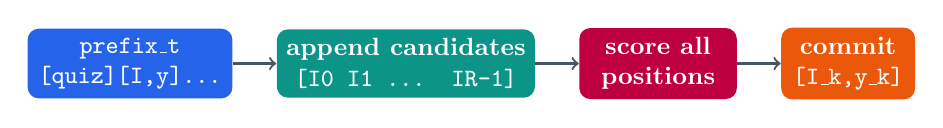
\begin{tikzpicture}[
      node distance=0.55cm,
      box/.style={rounded corners, draw=none, text=white, align=center, minimum height=0.78cm, font=\bfseries\small},
      arrow/.style={->, thick, draw=serslate}
    ]
      \node[box, fill=serblue, minimum width=2.6cm] (p) {\texttt{prefix\_t}\\ \texttt{[quiz][I,y]...}};
      \node[box, fill=serteal, minimum width=3.0cm, right=of p] (c) {append candidates\\ \texttt{[I0 I1 ... IR-1]}};
      \node[box, fill=purple, minimum width=2.0cm, right=of c] (s) {score all\\positions};
      \node[box, fill=serorange, minimum width=1.7cm, right=of s] (m) {commit\\\texttt{[I\_k,y\_k]}};
      \draw[arrow] (p) -- (c);
      \draw[arrow] (c) -- (s);
      \draw[arrow] (s) -- (m);
    \end{tikzpicture}
  \end{center}

  \vspace{0.4em}
  \begin{block}{关键不变量}
    候选 index token 共享同一个 logical frontier；每个候选可以看完整 prefix，但候选之间互相不可见。
  \end{block}

  \[
    prefix_{t+1}=prefix_t + [I_k, y_k]
  \]
\end{frame}

\begin{frame}[fragile]{原始 recompute 路径}
  \begin{lstlisting}
for step in range(R):
    idx_app = concat(prefix_t, all_index_tokens)
    logits = score_parallel_indices(idx_app, R)
    commit one [index, value]
    prefix_t = concat(prefix_t, [index, value])
  \end{lstlisting}

  \begin{itemize}
    \item 每一步重新 encode 正在增长的 \texttt{prefix\_t}。
    \item 每一步也重新 encode 全部 candidate index block。
    \item prefix 每步增长 2 个 token：\texttt{[index,value]}。
  \end{itemize}

  \vfill
  \small Code: \texttt{Ser-FOX/serfox\_model.py:728} \quad \texttt{score\_parallel\_indices}
\end{frame}

\begin{frame}[fragile]{当前 KV-cache 路径}
  \begin{lstlisting}
cache = build_prefix_kv_cache(prefix_0)

for step in range(R):
    logits = score_parallel_indices_cached(all_index_tokens, cache)
    commit one [index, value]
    cache = append_to_kv_cache(cache, [index, value])
  \end{lstlisting}

  \begin{itemize}
    \item prefix K/V 只构建一次。
    \item candidate block 仍然完整并行打分。
    \item 每步选中后，只把 committed \texttt{[index,value]} 追加进 cache。
  \end{itemize}

  \vfill
  \small Code: \texttt{build\_prefix\_kv\_cache:613}, \texttt{append\_to\_kv\_cache:638}, \texttt{score\_parallel\_indices\_cached:814}
\end{frame}

\begin{frame}[fragile]{同一个 visibility mask}
  \begin{columns}[T,onlytextwidth]
    \begin{column}{0.46\textwidth}
      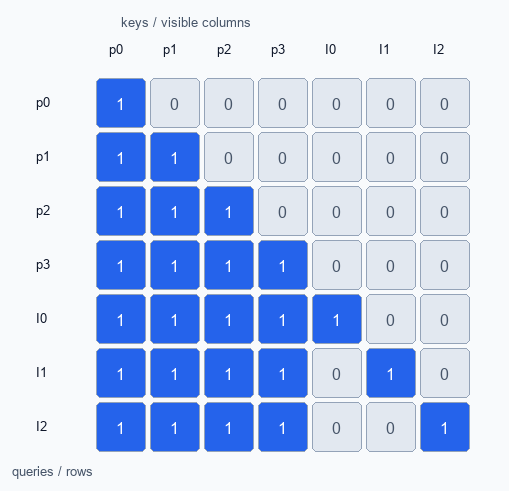
\includegraphics[width=\linewidth]{serfox_mask_matrix.png}
    \end{column}
    \begin{column}{0.50\textwidth}
      \begin{block}{Mask 规则}
        \begin{itemize}
          \item prefix $\rightarrow$ prefix：标准 causal lower triangle。
          \item candidate $i \rightarrow$ prefix：visible。
          \item candidate $i \rightarrow$ candidate $i$：visible。
          \item candidate $i \rightarrow$ candidate $j, i \ne j$：hidden。
        \end{itemize}
      \end{block}

      \begin{lstlisting}
visible = torch.eye(T)
# used when causal_new_tokens=False
      \end{lstlisting}
    \end{column}
  \end{columns}

  \vfill
  \small Code: \texttt{build\_ste\_visible\_mask:26}, \texttt{forward\_new\_tokens\_with\_kv:199}
\end{frame}

\begin{frame}{等价性计算}
  记 prefix cache 为：
  \[
    K_p,V_p = \mathrm{TransformerPrefix}(prefix_t)
  \]

  candidate block 投影为：
  \[
    Q_c,K_c,V_c = \mathrm{Project}(candidates)
  \]

  对任意 candidate row，recompute 路径计算：
  \[
    \mathrm{softmax}\left([Q_cK_p^\top,\; Q_cK_c^\top\ \text{masked-to-self}]\right)[V_p,V_c]
  \]

  KV-cache 路径计算同一个式子：
  \[
    \mathrm{softmax}\left([Q_cK_p^\top,\; Q_cK_c^\top\ \text{masked-to-self}]\right)[V_p,V_c]
  \]

  因此，令
  \[
    S_{\mathrm{full}}=\texttt{score\_parallel\_indices}(\cdot),\qquad
    S_{\mathrm{cache}}=\texttt{score\_parallel\_indices\_cached}(\cdot),
  \]
  则在同一 prefix 和 candidate block 下：
  \[
    S_{\mathrm{full}} \equiv S_{\mathrm{cache}}.
  \]
\end{frame}

\begin{frame}{速度提升来自哪里}
  \begin{columns}[T,onlytextwidth]
    \begin{column}{0.48\textwidth}
      \begin{block}{旧版}
        \begin{enumerate}
          \item recompute \texttt{prefix\_t + all candidates}
          \item commit \texttt{[index,value]}
          \item repeat with longer prefix
        \end{enumerate}
      \end{block}
    \end{column}
    \begin{column}{0.48\textwidth}
      \begin{block}{当前}
        \begin{enumerate}
          \item build prefix K/V once
          \item score candidates against cache
          \item append only \texttt{[index,value]}
        \end{enumerate}
      \end{block}
    \end{column}
  \end{columns}

  \vspace{0.7em}
  \begin{alertblock}{正确表述}
    KV-cache 加速的是 prefix accumulation，避免重复 encode 已经确定的 serialized prefix；PI candidate scoring 仍然是同一个并行打分问题。
  \end{alertblock}
\end{frame}

\begin{frame}{简单数值验证}
  \begin{columns}[T,onlytextwidth]
    \begin{column}{0.32\textwidth}
      \begin{block}{Setup}
        \begin{itemize}
          \item CPU only
          \item B=16
          \item 3 layers, 4 heads
          \item embd=128
          \item quiz=16, response=36
        \end{itemize}
      \end{block}
    \end{column}
    \begin{column}{0.32\textwidth}
      \begin{block}{Old vs current}
        \begin{itemize}
          \item max\_abs\_diff: \textbf{0}
          \item finite masks equal: \textbf{True}
        \end{itemize}
      \end{block}
    \end{column}
    \begin{column}{0.32\textwidth}
      \begin{block}{Recompute vs cache}
        \begin{itemize}
          \item max\_abs\_diff: \textbf{4.77e-07}
          \item finite masks equal: \textbf{True}
        \end{itemize}
      \end{block}
    \end{column}
  \end{columns}

  \vspace{0.7em}
  解释：cache 路径和 recompute 路径只有正常浮点误差量级差异。
\end{frame}

\begin{frame}{简单速度对比}
  \begin{table}
    \centering
    \begin{tabular}{lrr}
      \toprule
      Path & Median time & Relative \\
      \midrule
      old recompute & 1166.1 ms & 1.00x \\
      current recompute & 1168.0 ms & 1.00x \\
      current KV-cache & 937.7 ms & 1.25x faster \\
      \bottomrule
    \end{tabular}
  \end{table}

  \begin{itemize}
    \item current recompute 和 old recompute 基本同速。
    \item 加速来自 KV-cache 去掉重复 prefix encode。
    \item CPU toy benchmark 只作为方向性说明；正式 GPU/大任务需要单独 benchmark。
  \end{itemize}
\end{frame}

\begin{frame}{改了什么，没有改什么}
  \begin{columns}[T,onlytextwidth]
    \begin{column}{0.48\textwidth}
      \begin{block}{Changed}
        \begin{itemize}
          \item \texttt{build\_prefix\_kv\_cache}
          \item \texttt{append\_to\_kv\_cache}
          \item \texttt{score\_parallel\_indices\_cached}
          \item generation / regeneration can use cache path
        \end{itemize}
      \end{block}
    \end{column}
    \begin{column}{0.48\textwidth}
      \begin{block}{Did not change}
        \begin{itemize}
          \item single-index visibility rule
          \item candidate index isolation
          \item PI position-choice semantics
          \item candidate value logits surface
        \end{itemize}
      \end{block}
    \end{column}
  \end{columns}
\end{frame}

\begin{frame}{推荐对外说法}
  \begin{block}{Compact explanation}
    Our current code is an incremental implementation of the same PI scorer.
    The original code recomputed the entire serialized prefix plus all candidate
    index tokens at every step. The new code caches the prefix K/V once, scores
    the same candidate index block against that cache using the same
    index-isolating visibility mask, and after selecting one position appends
    only the committed \texttt{[index,value]} pair. Therefore the mathematical
    scorer is the same; the speedup comes from eliminating repeated prefix
    computation.
  \end{block}

  \begin{alertblock}{Caveats}
    \texttt{use\_rope=True} and grouped-index scoring are new optional paths.
    \texttt{norepeat} / \texttt{pad\_eos\_last} are decode-time logit masks, not
    attention masks.
  \end{alertblock}
\end{frame}

\end{document}
